\documentclass[12pt,a4paper,oneside]{article} %% Dokumenten Parameter und Art des Dokuments
\usepackage[utf8x]{inputenc} %% Diese Datei ist im utf8 Format dies ist hier damit Latex uns versteht
\usepackage[ngerman]{babel} %% Rechtschreib prüfung
\usepackage{hyperref}
\usepackage{amsmath} %% Packet zur verwendung Mathematischer Formeln
\usepackage{amsfonts}
\usepackage{amssymb} %% Packet zur verwendung Mathematischer Symbole
\usepackage{mathtools}
\usepackage{microtype} %% Sorgt für besseren umgang mit zu lange/kurzen Zeilen
\usepackage{pdfpages} %% Zum einfügen eines PDf dokuments
\usepackage{pgfplots}

\title{Fuzzy Serie 10}
\author{Bennet Bleßmann, Bennet Krause}

\begin{document}
\maketitle

\setlength{\parindent}{0pt}
\section*{\underline{Aufgabe 19}}

\subsection*{a)}

Das ANFIS-Modell hat genau wie das Modell aus Aufgabe 18 vier Regeln.\\

% train error: 0.39521
% check error: 0.44638

Der Fehler für die Trainingsdaten beträgt $0.39521$. Der Fehler für die Checking-Daten ist mit $0.44638$ etwas höher.

%TODO vergleich mit errors aus A18 

\subsection*{b)}

Dieses Modell besitzt 32 Regeln, gegenüber den nur vier Regeln aus a) und Aufgabe 18.\\

% train error: 0.03301
% check error: 7.9124

Die Genauigkeit ist auf den ersten Blick viel besser als in a). Der Trainingsfehler beträgt nur $0.03301$. Sieht man sich die Visualisierung an, kann man sich aber denken, dass die Übereinstimmungen wahrscheinlich etwas zu präzise sind und das Modell starkes Overfitting aufweist, sich also exakt auf die Trainingsdaten eingestellt hat:\\

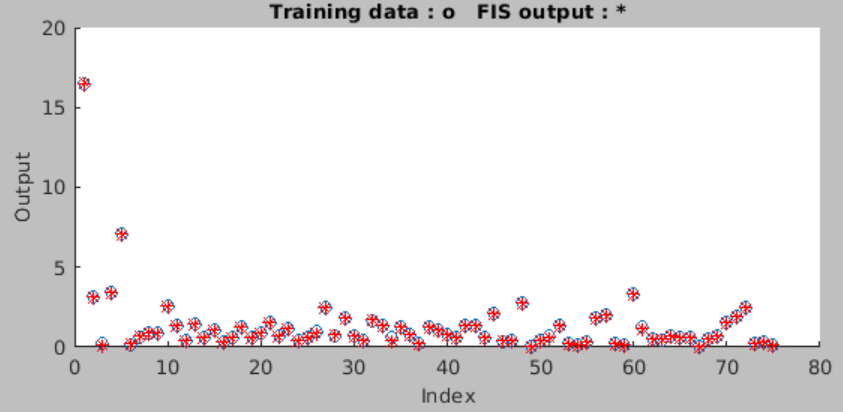
\includegraphics[width=\textwidth]{part/grid_train.png}\\

Und tatsächlich beträgt der Fehler auf den Checking-Daten $7.9124$ gegenüber dem viel kleineren Fehler von $0.44638$ in a).

%TODO vergleich mit errors aus A18 	
\end{document}